\chapter{Question-Asking and Plan Inference}
\label{ch:question_plan}
\textbf{Salena Torres Ashton, Stephen Kim, Loren Rieffer-Champlin, Liang Zhang,
Adarsh Pyarelal, Clayton Morrison}
%% Start on line 115

\section{Summer 2022 Introduction}
\subsection{Significance of Question-Asking in SAR Scenarios}
When we share information\footnote{The Introduction and Evaluation sections of this chapter have been significantly rewritten. To maintain transparency, the Approach section has remained as written in the preregistration. As a consequence, some redundancy may be found between sections.}, clarify ambiguity, or optimize instruction execution, we often do so through question-asking and question-answering. This mode of communication often reflects our intention, strengthens relationships, increases productivity, reduces risk, and creates an equitable environment \citet{rothe_lake_gureckis_2018} and \citet{alaimi_2020} between dialog partners. In the SAR scenario implemented for ASIST Study 3, teams of human players engage in cooperative behavior to search for, stabilize, and rescue victims within a collapsed building. As human players verbalize plans, make suggestions, or tell each other what to do, they also ask questions that can infer hidden goals or intentions. Question-asking enables teammates to reduce their individual knowledge asymmetry.  

Not understanding a goal or intention can be seen in the designs of artificial intelligence agents that may have been programmed with researcher bias. If that AI agent's purpose is to assist humans in a SAR scenario, the programmer and researcher must check (or augment) their own domain knowledge of SAR communications in order to curb potential bias toward academic best practices regarding the programming of uncertainty, belief and reinforcement learning. Understanding SAR communications facilitates programmers to design a realistic and scalable domain; not doing so, or at least not consulting SAR experts regarding their information-gathering and sharing habits, can result in flawed domains that predict human player and AI agent action at no better than chance. 

Therefore, question-asking and information-sharing is vital in a domain definition of a Search and Rescue scenario (SAR)  as much as it is in real life. The INSARAG marking system\footnote{FEMA has a similar marking but is only used in the United States, whereas INSARAG is used internationally.} is designed to immediately answer the most frequently-asked questions a rescuer will have in an urban SAR disaster: Go or No-Go, number of live victims, number of dead victims, number of unaccounted-for victims, hazards, building floor references, cleared areas of building, and cleared building \citet{insarag_2022}. SAR workers further communicate with each other through radio, sound horns, Morse code, and direct communication with victims and each other.

This registration investigates the gap between question-asking in natural language discourse and player goals through goal inference. In the SAR scenario implemented for ASIST Study 3, teams of human players engage in cooperative behavior to search for, stabilize, and rescue victims within a collapsed building. As human players verbalize plans, make suggestions, or tell each other what to do, they also ask questions that can infer hidden goals or intentions. Using procedural Grounded Theory to annotate video observations of teams who play Minecraft in an urban search and rescue scenario, we then map players' utterances to action and intention. Actions and intentions are then mapped into action and task definitions of the HDDL declarative language\footnote{See previous section, written by Loren Champlin et al for a description of HDDL and our plan recognition development.} The results of this study show that teams who ask more questions at a more consistent rate lead to better team performance than teams who ask fewer questions, ask more how-to questions, or use questions as a polite way to give directions to teammates. The registration concludes with suggestions for further research development regarding the knowledge engineering and representation of tasks, goals, and hidden intentions. While simple human goals may be represented with classical AI planning, we believe that complex goals with constraints or multiple levels of abstraction may be best represented by a \emph{hierarchical task network} (HTN)\ap{Add a definition of HTN here}, which is a tree of possible plans.\footnote{Technically, the plans produced by HTN planners can also be represented with flat lists - however, in this section, we use the term `plan' to refer to the actual `plan tree' that contains the task decompositions
as well, rather than just the plan alone.}

\begin{enumerate}
    \item How do spoken questions reveal another person's plan or intent? 
    \item Can people listen to spoken questions and accurately decide if the other person's plan is sequential or hierarchical? Can the distinction between such structures improve predictive performance for Artificial Social Intelligence (ASI) agent intervention?
\end{enumerate}

Artificial Intelligence (AI), Information Retrieval, and Natural Language Processing yield exciting research into question-\emph{answering}, relevant document retrieval, Theory of Mind (ToM), and human-computer interaction. However, the literature is sparse within the  \emph{intersection} of artificial intelligence, psycho linguistics, indirect speech acts, negative knowledge modeling, ToM, and question-\emph{asking}. Hawkins and Goodman address this sparsity and the trend of past research to focus on the optimization of question-answering, not question-asking \citet{hawkins_goodman_2017}. 

\subsection{Literature}
When we ask questions, we are not seeded with a set of questions or handed a set of 'correct and incorrect' questions. We do not prefer questions with literal, logical answers \citet{rothe_lake_gureckis_2017} and \citet{clark_1979}. However, most research has focused on answer sets or query matching, preference for concise questions and answers. In reality, people ask open-ended questions, sloppy half questions, use questions to politely tell others what to do, and meander in speech without purpose \citet{brown_1980}. We ask questions to express goals. 

Goals reflect a desired endpoint or world state. A goal can be motivated by belief, desire or intent. People ask questions that either express a goal or infer a hidden goal. A question is the interpretation and response of a hidden (or uttered) goal to be discerned
by another person, typically a dialog partner \citet{hawkins_goodman_2017}. Indirect speech acts and question-answer dialog is a form of \emph{information asymmetry}: a questioner has a goal but needs information, while an answerer has information but does not know the questioner’s goal. Missing or contradictory information naturally leads to a knowledge goal and the generation of questions. The person is then motivated to ask a question \citet{alaimi_2020}. 

Intentions demonstrate action choice to reach that goal-- it is reflected in the way a question is to be asked. A questioner believes that the listener’s knowledge base has information that can facilitate the questioner’s goal.  The type of questions then asked will depend on context, social inference, and other signals in a dialog setting. The key is to decouple\footnote{Hawkins and Goodman's 2017 work was limited to epistemological questions and cooperative behavior.} the inferred goal from the explicit meaning of the question \citet{hawkins_goodman_2017}. This redefinition of \emph{What is a Question} enables models to account for context and avoid assumptions. 

Questions can be viewed as a hidden goal or intent, but they can also be viewed as a way to provide or reinforce knowledge \citet{alaimi_2020} and \citet{ray_2001}. Question-askers want the listener to directly understand their goal, or to discern a hidden goal, or both-- then to give appropriate responses (however that appropriate response may be for the context). When question-askers do not receive appropriate answers from listeners, both dialog partners use conversational implicature and politeness to reach a mutual understanding. They will minimize potential transaction and opportunity costs in conversation to reach mutual understanding.  




\section{Approach}

We assume that questions have hidden goals and infer plans. As teams ask more
questions of each other, human team ToM converges toward cooperative behavior.
We will investigate whether question-asking is associated with \emph{team
planning}, defined as a set of goals, strategies, or tasks that are executed.
We define \emph{coordination} as behaviors and utterances to create a common
plan or strategy\footnote{Note that this is distinct from the mathematical
definition of coordination proposed in \autoref{ch:pgm}}. We define
\emph{cooperation} as team behaviors that implement an already-agreed up on
plan.

To capture hidden goals, inferred plans, and patterns that may represent human
ToM, we will annotate six ASIST Study 3 Spiral 2 pilot video observations and
six HSR ASIST Study 3 videos released between March 29 and May 5, for a total
of at least twelve videos. These videos are of three distinct missions for each
team. Due to the expensive costs of taxonomy label development with strict
adherence to grounded theory methodology, this stage of the experiment is
limited to no less than twelve videos. 

Two human annotators will code all uttered questions between teammates within
the Minecraft SAR scenario.  We use the qualitative coding procedure known as
Grounded Theory, as defined by \citet{corbin_strauss_2015}. 

More specifically, and as defined by \citet{saldana_2021}, we will use a
Grounded Theory Process Coding for a state or action across some interval of
time. These \emph{grounded-in-data} labels are known as \emph{concept-level}
labels, which are the smallest pieces of data that encode a question-asking
phenomena of interest.

More specifically, and as defined by \citet{saldana_2021}, we will use a
Grounded Theory Process Coding for a state or action across some interval of
time. These \emph{grounded-in-data} labels are known as \emph{concept-level}
labels, which are the smallest pieces of data that encode a question-asking
phenomena of interest. We also use this coding methodology to investigate the connectivity and
causality of each concept label to discover possible relationships between
presence or absence of team actions, interactions, conditions, and consequences
of question-asking. Densely-connected concept labels suggest subcategories and
categories. Sparsely-connected labels will not be discarded; they will be used
to consider variability within patterns and categories that emerge. In cases
where questions have co-reference or other contextual dependencies, only that
direct dependency will be coded for local semantic meaning.

We make the following considerations when creating codes: 

\begin{itemize}
    \item Frequency will not dictate importance, causality, or connectivity of a concept
    \item Each question will have at least one annotation and up to four
      annotations:
    \begin{itemize}
        \item Primitive actions (ground truth). Ex: breakRubble,
          requestStabilizedVictimCarry.
        \item Abstraction Levels of actions (of primitive actions) Respective
          examples: respondRubbleRequest or createVictimAccess, collaborateStabilizedVictim
    \end{itemize}
    \item Labels will be stemmed and minimally normalized
    \item Capturing the phenomena of question-asking across time, between any subset of a team, between the same team across the two different missions. 
\end{itemize}


To avoid annotator and researcher biases and any \emph{a priori} belief on
which team ToM strategies may be used, concept and category labels are not
pre-determined. Inter-annotator agreement must reach a Kappa Score of 80\% or
higher. This also gives a more solid, grounded analytical meaning to any
emergent categories. 

After the development of labels and taxonomy, the investigation of team ToM and
question-asking will scale for additional videos. When all concepts,
subcategories, categories can reasonably explain the phenomena of the video
observations, one or two super-categories, \emph{theories of team plan}, will
emerge. We currently assume that a theory of team plan would have greater
predictive power and ToM inference potential. 





%% Start here

\section{Evaluation}
\subsection{Label Development and Kappa Score}
The results of this study show that teams who ask more questions at a more consistent rate lead to better team performance than teams who ask fewer questions. When teammates ask each other questions, they engage with each other more often, evidenced by the rescue of critical victims (which require teamwork) as opposed to regular victims (which can be done individually). The data warrant further research into question-asking, information-sharing, and knowledge asymmetry between dialog partners.

To capture hidden goals, inferred plans, and patterns, twelve ASIST Study 3 video observations were annotated\footnote{Due to the expensive costs of taxonomy label development with strict adherence to Grounded Theory methodology, this stage of the experiment is limited to twelve videos.}. Videos were annotated using a bottom-up Grounded Theory qualitative coding method to investigate connections between a question-asker's intention and words spoken. This rigorous theory ensures that the labeling is not biased, as it uses unsupervised labels and does not lend itself to the proof or disproof of prior researcher
belief in Minecraft SAR player strategy. This data-driven, robust method captures player intention, team strategy, and naturally lends itself to
quantitative analysis. Videos were selected from no-human intervention videos, at random, and three teams were chosen as a sequence (team 217, 218 and 219).
Two independent annotators\footnote{Salena Ashton, PhD Student, School of Information, University of Arizona; and Stephen Kim, MS Information Science} annotated the videos with unconstrained, not-previously-determined labels and were free to create any label desired to code a
player's question.

The continuous disambiguation of unsupervised labels, using lexical definitions, led to extensive
documentation of words to be used as labels for the capturing of specific phenomena in observations\footnote{Salena Ashton and Loren Reiffer-Champlin, both PhD Students, School of Information, University of Arizona.}. This lead to Theoretical Saturation\footnote{Theoretical saturation is the point when few additional labels are created, regardless of fully-autonomous annotators' ability to create new ones. Saturation demonstrates that the existing label schema fully capture the events and phenomena observed.} and the labeling schema converged to 21 verb
labels, 24 noun labels, 25 modifier labels. Without replacement, these
components can yield 12,600 possible labels, yet demonstrated theoretical
saturation through the independent construction of less than 100 labels from the 
two autonomous annotators.

An unweighted Cohen Kappa\footnote{Grounded Theory is robust in its
unsupervised labeling approach is because annotators have complete autonomy.
Because the sample size is small, the theoretical probability of two matching
labels is even smaller, and only two annotators worked on the real data, there
is no current justification for using Scott's pi or a weighted Kappa. This will
change as further research scales.} agreement of 0.892 was achieved. Using the
disambiguation documentation and Merriam-Webster's Dictionary to meticulously
settle any annotator label disagreement, question labels were declared as
'agree' or 'disagree'. When annotator intention and the disambiguation
documentation did not clarify the agreement or disagreement of labels, the label was labeled as 'disagreement.'

Overall, about 100 labels resulted and were analyzed for
emergent categories and preliminary patterns. Label frequency \textit{did not}
dictate importance. Data visualization and preliminary analysis focus on three
key features: \textit{questionLabel}\footnote{Qualitative code representation of the
question utterance and no further context except for co-reference resolution.
Some questions were spoken as statements with inflection. Other questions were
actually demands shrouded with politeness. All three types of questions were
coded for this investigation. All questions asked are assumed to be uttered
with cooperative intent.}, \textit{abstractLabel}\footnote{Code representation of
player intention. This was captured by taking the question into context. For
example, if the question were represented by 'requestBreakRubble', the intent
behind the question could have been 'collaborateCriticalWake' or
'navigateLocation'. AbstractLabel is not the representation of *why* a
question had been asked; it is the *intention* of the player who asked the
question.}, and \textit{utterance}, the word of interest uttered in a question. From
the emergent categories, specific words were chosen that did or *did not*
represent player interaction\footnote{For example: *ask*, *request*,
*suggest*, and *clarify* are all actions that show the goal of
obtaining information, but 'clarify' asks for additional information after the
initial question, showing two-way dialog, 'request' is an initiation of
commitment to another player with the optional accept/ reject response, showing
two-way dialog. 'Suggest' also initiates like 'request' but does not give the
option to accept or reject, making the question and dialog a one-way
discussion. 'Ask' is a one-way dialog utterance to obtain information.}. 


\subsection{Emergent Categories}


The following themes emerge from the data:

\begin{itemize}
    \item Less Team Collaboration (talking \emph{at or to} a teammate and not \emph{with} a teammate)
    \begin{itemize}
    	\item Labels that include: direct, suggest, inform, etc.
	\item Word utterances: go, I see, there are, and other phrases that inform but do not invite collaboration
    \end{itemize}
    \item More Team Collaboration (talking \emph{with} a teammate)
    \begin{itemize}
        \item Labels that include: ask, request, answer, clarify, teammate, coordinate, collaborate, plan, wake
        \item Word utterances: can you, should we, you guys, what do you think, let's, wake, this time
    \end{itemize}
    \item Intention toward position: location or destination, but not necessarily navigation strategies.
    \item Prioritizing an idea: plan, suggest, request, collaborate, critical, or any victim.
    \item Question utterances that were actually demands (do you mind doing...; why don't you go and clear...). This indicates conversation implicature and politeness, as described by the Gricean Maxims and Gretchen Brown.
    \item Statements that were questions with inflection, and other nuanced utterances: suggest, tell, direct, request; context and explanations included in annotation.
\end{itemize}



Teams who scored higher tended to ask questions about the collaboration of victims, whereas teams who did not score as high asked questions about location or destination (where destination is a location that is a goal). Player intention (represented by abstract labels) is an unobserved, inferred behavior. Teams scored more points when they tended to rescue critical victims more often than regular victims. A critical victim requires that at least two players of the team are present to "wake" up the victim, then another team player will heal the victim. This collaboration more often results from teams who speak with each other and make more verbal requests of each other to help wake up the critical. In fact, the most common question that was verbalized centered on the idea of requesting a teammate to come to a particular destination.

The general trend of teams working together to score higher points: teams must work together to rescue critical victims, who cannot be saved by only one player. Teams who asked more questions and worked together tended to save more critical victims and score higher points. While it is possible for teammates to rescue critical victims without asking questions or verbalizing any type of request, it is difficult due to the time constraint of the mission (15 minutes). 


Teams who scored more points not only asked more questions, but tended to ask questions that invite collaboration. Question that begin with "Do/ does/ did" or "when/ where", and "what" indicate questions that require a response from another teammate. 

Non-trivial amounts of questions are, in fact, imperative statements with added inflections at the end; asking questions as if they were questions but are actually disguised imperatives. For example, "Take this victim, will you?" does not invite the listener to accept or deny this request. Likewise, "You'll take this victim," with inflection at the end of the sentence \textit{sounds} like a question, but is also an imperative. 






\newpage
\section{Preliminary Conclusions with Figures}
Teams who scored higher tended to ask questions about the collaboration of victims, whereas teams who did not score as high asked questions about location or destination (where destination is a location that is a goal).



\begin{figure}[h!]
    \centering
    \fbox{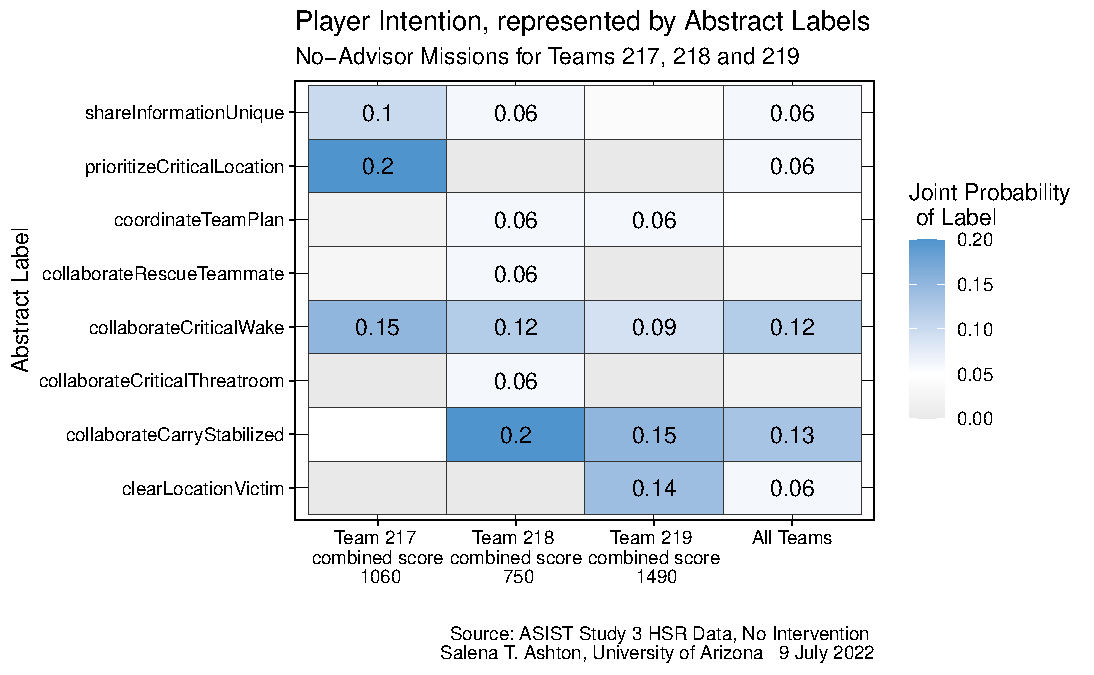
\includegraphics[width=0.9\textwidth]{../images/abstractLabelProbability_STA.pdf}}
    \caption{Player intention (represented by abstract labels) is an unobserved, inferred behavior. Ground-truth question utterances demonstrate team collaboration differently than abstract labels.}
\end{figure}


When we look at the question that was asked, we are able to predict their intentions only part of the time. Though we cannot conclude that questions will always predict intention from this small study, we can see that further research with a larger sample size is warranted. Patterns that emerge include that given question utterance 'requestDestination', the player's intent is more than 80\% likely to be waking a critical victim. Human annotators intuitively agree with this assessment.






Questions Asked, given the Player Intention: Three player intention themes emerge when all possible intentions are filtered for more than 10\%: collaborateCarryStabilized, collaborateCriticalWake, and prioritizeCriticalLocation. When a player's intention is to wake a critical, they are 55\% likely to ask another player to join
 them ('requestDestination'). This observation is trivial because the game rules state that at least two people are needed to wake a critical. However, the previous figure shows the flipped conditions: a player's intention is more than 80\% likely to be waking a critical when 'requestDestination' is asked. When teams collaborate to wake a critical victim, they request or clarify --not suggest or tell-- a teammate to come to a particular destination. ('Clarify' and 'request' infer two-way dialog of commitment creation whereas 'direct' or 'suggest' are creation commitments or demands that do not give the listener a chance to respond.) 








\begin{figure}[h!]
    \centering
    \fbox{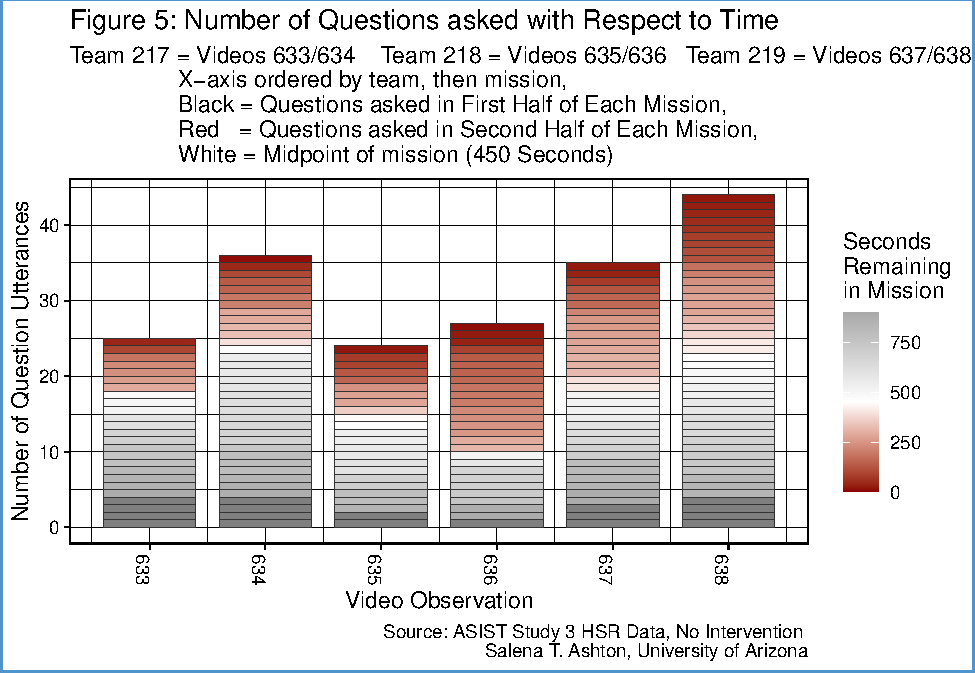
\includegraphics[width=0.9\textwidth]{../images/QuestionTiming_STA.pdf}}
    \caption{Time is displayed as color, where dark gray is at the beginning of the mission and red is toward the end of the mission. Team 218 (videos 635 and 636) asked the
fewest questions, scored the lowest combined points, and asked 66\%
of questions toward the end of the mission. This suggests that teams who score poorly tend to ask fewer questions that focus on collaboration or planning-- and more questions that ask specific task-oriented items toward the end of each mission. Team 3 (videos 637 and 638) asked the most questions and asked questions at a \emph{consistent rate} throughout their missions. This suggests that teams who score higher tend to ask questions at a consistent rate, enabling the exchange of information, building of rapport and team trust, and setting a social convention of asking each other for collaboration or help. }
\end{figure}






\begin{figure}[h!]
    \centering
    \fbox{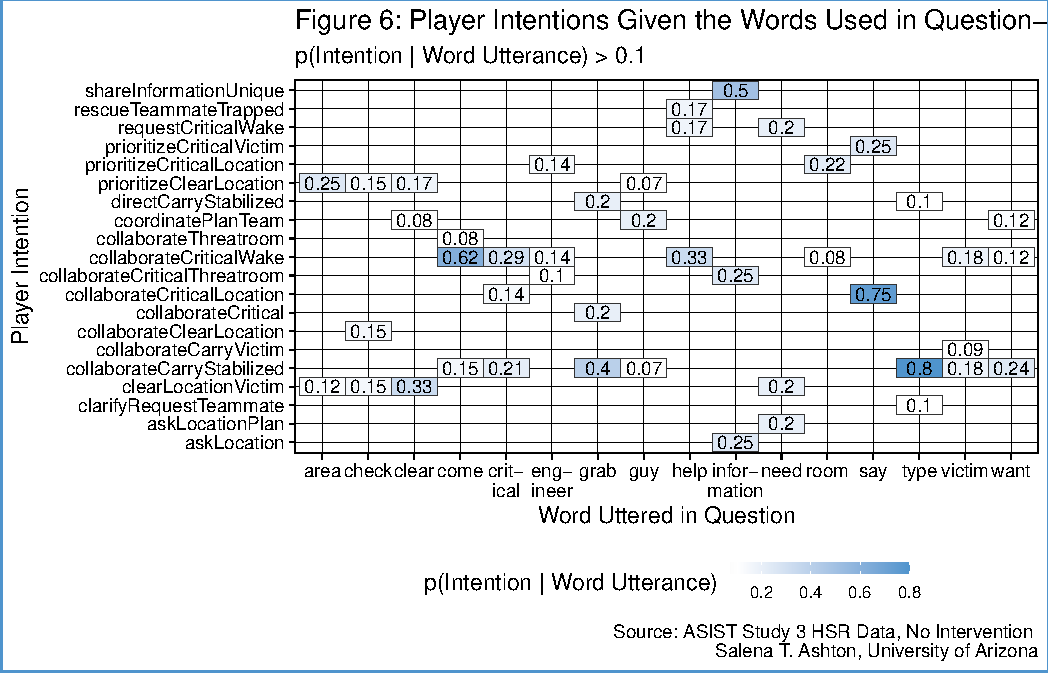
\includegraphics[width=0.9\textwidth]{../images/QuestionUtterances_Link_STA.pdf}}
    \caption{Non-domain-specific words that show collaboration include: say, type, or come. These conclusions were made using the 1 x 1 Bag of Words algorithm and matched to intention by hand. The \textbf{significance} of this figure shows that a priori researcher bias can be harmful when designing a domain. For example, our team previously believed that words like: navigate, location, victim, room, critical and marker were the most important words to look for when inferring player intention. This figures shows that is not the case. A priori research team error: navigate, location, victim, room, critical, marker, or area.}
    \end{figure}
    
   
\begin{comment}
Corrected research team information regarding Player Intention:
\begin{itemize}
    \item 'Come' infers team collaboration for waking up a critical victim
    \item 'Grab' infers team collaboration for carrying victims that have been healed
    \item 'Say' infers team collaboration of locating critical victims
    \item 'Type' infers team collaborating for carrying victims that have been healed
\end{itemize}
\end{comment}




Word Utterance, given Player Intention: Players who work together tend to say  'come', 'say' (stemmed), 'type' or 'want.' When they work together to carry victims, they will most likely say 'type' (or mark) to identify the victim type. As shown, the emergence of a possibly-interesting pattern, especially when non-domain words like 'type' show a strong correlation to specific intentions. The \textbf{significance} of this figure demonstrates how plan-recognition researchers may consider such non domain-specific words when designing a domain.



The ultimate goals of this registration are two-fold: find evidence to (1)
continue the investigation of intent, given a question being asked, using
causal reasoning and other approaches (2) develop algorithms to extract this
intent from utterance transcriptions of player without human annotator
dependency. We believe that emergent categories that result from these 12 video
annotations do *warrant* continued investigation, which would include the
following possible tasks:

\begin{itemize}
    \item Scale for additional data: Ashton is currently building a model that maps words\footnote{Bag of Words and other models, at word and sentence level.} and intentions.
    \item Natural generation model: Use the above model to re-create the labels
        generated by Ashton and Reiffer-Champlin. We will compare these results
        to model labels with the taxonomy developed by ODIN and the Dialog
        Agent at the University of Arizona.
    \item Additional human annotation of data; compare models in earlier stages to these results until the automation of linking intention with natural language is credible and reproducible.
    \item Compare and contrast emerging team ToM from no-intervention observations to high-intervention observations.
    \item Quantitative analyses and causal inference models.
\end{itemize}



\begin{figure}[h!]
    \centering
    \fbox{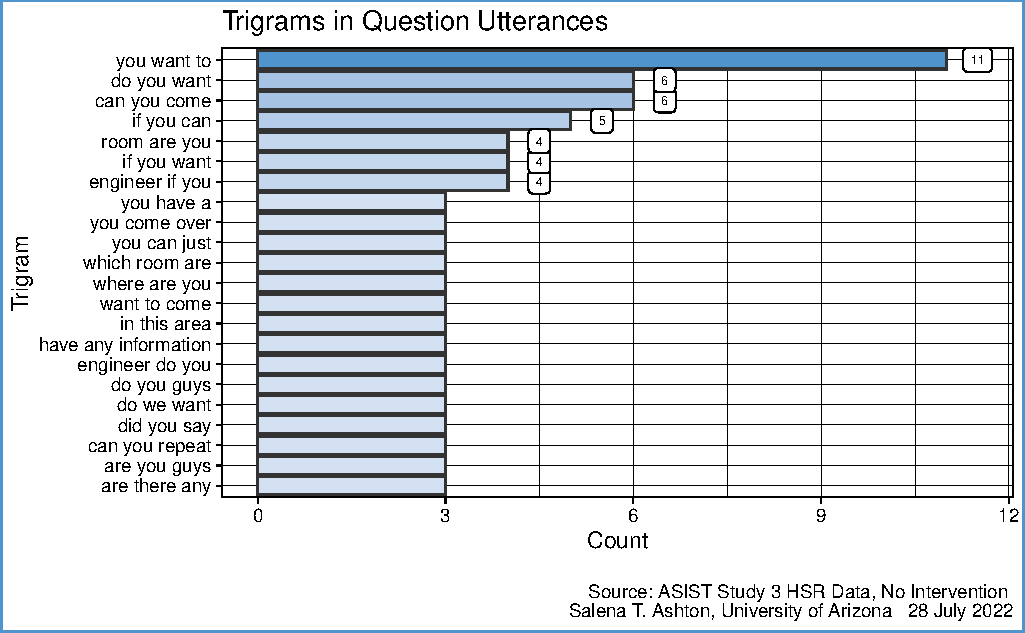
\includegraphics[width=0.9\textwidth]{../images/trigram_Utterances_STA.pdf}}
    \caption{Using the Python package NLTK, I extracted the most common N-grams of the players' question utterances (for all teams, N = 3). When I first did this, there were no interesting patterns. I then removed the "English" library of stopwords to be removed and found the following patterns. This yields exciting potential for further research into the logical argument and flow of player intention. For example, the word "if" shows a conditional statement from one player to another. "If you can..." was a common utterance but it was also a polite imperative, not a request or question. The phrase "do you guys" and "do we want" to not carry as much information about named entities, but it does show ample collaboration of teammates. }
\end{figure}

\begin{figure}[h!]
    \centering    
    \fbox{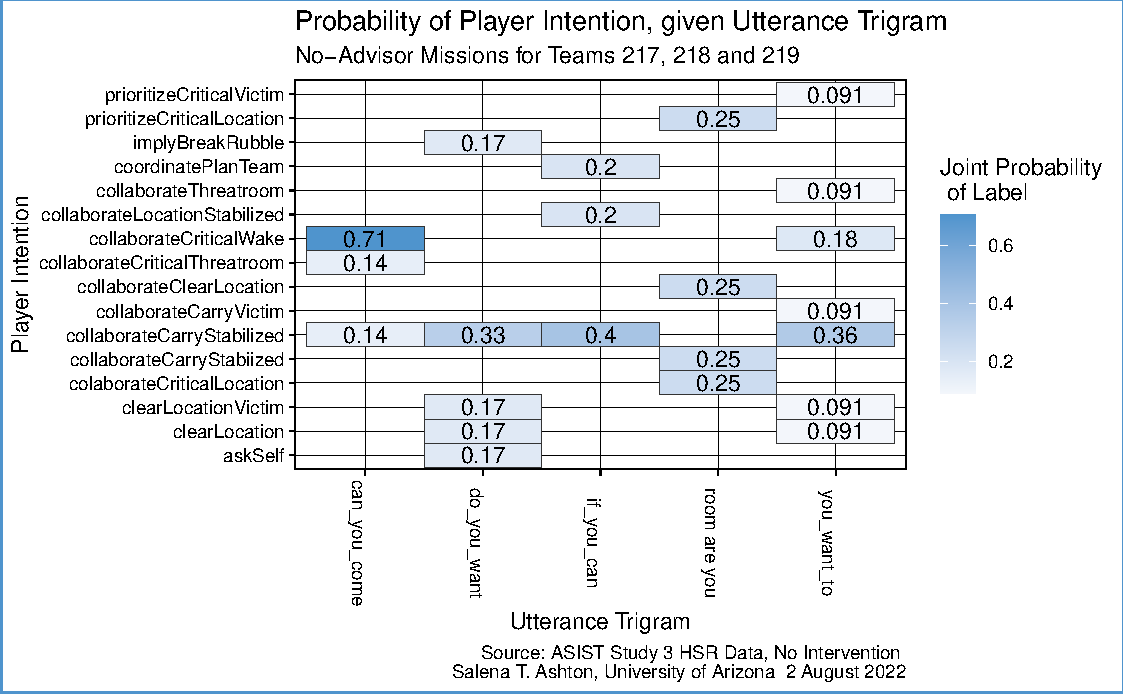
\includegraphics[width=0.9\textwidth]{../images/FINAL_1_trigram_Utterances_STA.pdf}}
    \caption{Probability of Player Intention, given Utterance Trigram}
\end{figure}





\subsection{pasted notes}
a player's intention is more than 80\% likely to be waking a critical when 'requestDestination' is asked. When teams collaborate to wake a critical victim, they request or clarify --not suggest or tell-- a teammate to come to a particular destination. ('Clarify' and 'request' infer two-way dialog of commitment creation whereas 'direct' or 'suggest' are creation commitments or demands that do not give the listener a chance to respond.)


\newpage

In this paper, I have discussed how questions can infer explicitly-stated goals, inferred goals, and how questions are better understood through indirect speech acts. I then use a Search and Rescue scenario within ASIST's Minecraft Environment to evaluate how teammates will ask each other questions in order to make and reach individual and team goals. These goals and player intentions were captured with a robust and vigorous coding process called Grounded Theory, annotated by two completely-autonomous annotators, and reached an unweighted Kappa Cohen score of 0.892. I then investigated these data through a series of visualizations, joint and conditional probabilities, and mapping the data to natural language utterances. This preliminary study has two significant limitations: Only twelve videos were annotated for questions. Future research must include the annotation of many more videos, their questions and non-questions. 

\subsection{Significant findings}
\begin{itemize}
    \item Previous researcher belief that players create intentions around domain-specific words are not supported in this research
    \item Previous top-down domain definition of the Search and Rescue yielded results that were no better than chance. This preliminary study shows several inferences that fair better than chance for player intention, questions asked, and natural language of questions that are asked.
    \item Teams demonstrate collaboration through non domain-specific words like 'come', 'say' and 'type'.
    \item Stops words that are traditionally removed for natural language processing must be considered when infering goals or intentions toward team collaboration. Furthermore, it is these stop words that show the logical inference of such plans.
\end{itemize}

\section{Discussion}

The data collected for this experiment were collected to answer the questions about goal, intention, and question-asking for team players within the virtual environment of a SAR scenario. The data were evaluated to see how teammates will ask each other questions in order to create team goals. These goals and player intentions were captured with a robust and vigorous coding process called Grounded Theory, annotated by two independent and autonomous annotators. Labeling reached an unweighted Kappa Cohen score of 0.892. Using this data, this paper answered three particular questions:
\begin{itemize}
    \item Are teams more likely to score higher when they focus on critical or regular victims?
    \item Do teams who score higher ask more questions?
    \item What types of questions were most frequently asked?
 \end{itemize}

Teams require more collaboration and effort to save critical victims than when saving regular victims; those who ask more questions invite team collaboration and tend to score higher than teams who do not work together. The most common types of questions that teammates asked, given that they scored better than other teams, tended to questions that invited a response. Such questions started with "do", "can", "what", and "which". Common questions which did \textit{not} result in high scores tended to start with "have", "is", and "were". These questions were more about information-seeking than team collaboration.
 
This preliminary study has two limitations: Only twelve videos were annotated for questions. Further research is warranted for the investigation of question-asking, goal-setting, goal-reaching, and team collaboration. Using the current label taxonomy, future research is scaleable and can include the annotation of questions and imperative statements. 



\subsection{Future Research}
I have found that further research is warranted for the investigation of question-asking, goal-setting, goal-reaching, and team collaboration. As a bonus, I have discovered that the stop-words not only hold potential research investigation for the logical flow of such arguments, but can possibly yield new insight into causal inference and reasoning\footnote{It is my intention to continue this line of research for a directed research study in Fall 2022 (Causal Inference) and in Spring 2023 (Comprehensive Qualification Exam for my PhD program in Information Science at the University of Arizona).} It is my hope that the findings of this preliminary study and future research will have significant application toward continued work for the ToMCAT- ASIST program \footnote{Theory of Mind-based Cognitive Architecture for Teams (ToMCAT), Natural Language Generation for Artificial Intelligence and Planning Task \# 7} and for continued study of probabilistic and causal reasoning. 

This future investigation would
address measure ASI-M5: Coordinative Communications to
measure teamwork, include additional video observations for real data in Study
3, and continue our investigation of whether human plans and ToM are best
represented by classical planning or HTN planning.

\newpage





